\documentclass{article}%
\usepackage[T1]{fontenc}%
\usepackage[utf8]{inputenc}%
\usepackage{lmodern}%
\usepackage{textcomp}%
\usepackage{lastpage}%
\usepackage{geometry}%
\usepackage{float}%
\usepackage{caption}%
\usepackage{xcolor}%
\usepackage{graphicx}%
\usepackage{multicol}%
\usepackage{listings}%
\usepackage{tikz}%
\usepackage{pgfplots}%
\usepackage{tcolorbox}%
%
\usepackage[utf8]{inputenc}%
\usepackage[T1]{fontenc}%

        \lstset{
            basicstyle=\ttfamily\small,
            frame=single,
            breaklines=true,
            numbers=left,
            numberstyle=\tiny,
            keywordstyle=\color{blue},
            commentstyle=\color{green!50!black},
        }
        %
\graphicspath{{images/}}%
\title{Reporte Técnico ViewX}%
\author{Emmanuel Ascendra}%
\date{\today}%
%
\begin{document}%
\normalsize%
\pgfplotsset{compat=1.18}%
\maketitle%
Este reporte demuestra todas las capacidades del motor ViewX.\newline%
%
\textbf{Texto importante en negrita.}%
\section{Introducción}%
\label{sec:Introduccin}%
ViewX es un motor de generación de reportes científicos capaz de producir documentos profesionales usando Python.

%
\subsection{Características principales}%
\label{subsec:Caractersticasprincipales}%
\begin{itemize}%
\item%
Texto estructurado%
\item%
Imágenes%
\item%
Tablas%
\item%
Código%
\item%
Gráficos científicos%
\item%
Multicolumnas%
\item%
Cajas de información%
\end{itemize}

%
\section{Tabla de resultados}%
\label{sec:Tabladeresultados}%
\begin{table}[H]\centering
\caption{Comparación de modelos}
\begin{tabular}{l | l | l}\hline
Modelo & Accuracy & F1\\ \hline
Regresión & 0.82 & 0.79\\ \hline
Árbol & 0.91 & 0.88\\ \hline
Red neuronal & 0.94 & 0.92\\ \hline
\end{tabular}\end{table}

%
\section{Visualización}%
\label{sec:Visualizacin}%


\begin{figure}[H]%
\centering%

\includegraphics[width=0.6\linewidth]{Python-Emblem.png}%
\caption{Imagen de prueba}%
\end{figure}

%
\section{Código de ejemplo}%
\label{sec:Cdigodeejemplo}%

    \begin{lstlisting}[language=python]
    
import numpy as np

x = np.linspace(0, 10, 50)
y = np.sin(x)

    \end{lstlisting}
    

%
\section{Análisis en dos columnas}%
\label{sec:Anlisisendoscolumnas}%
\begin{multicols}{2}%
Este bloque demuestra cómo dividir el contenido en múltiples columnas dentro del mismo documento.%
\begin{itemize}%
\item%
Ideal para papers%
\item%
Mejora lectura%
\item%
Ahorra espacio%
\end{itemize}%
\end{multicols}

%
\section{Nota importante}%
\label{sec:Notaimportante}%

\begin{tcolorbox}[
    colback=green!20,
    colframe=black,
    title=Observación clave
]
Todos los elementos se generan directamente desde Python.
\end{tcolorbox}

%
\section{Gráfico simple}%
\label{sec:Grficosimple}%

\begin{figure}[H]
\centering
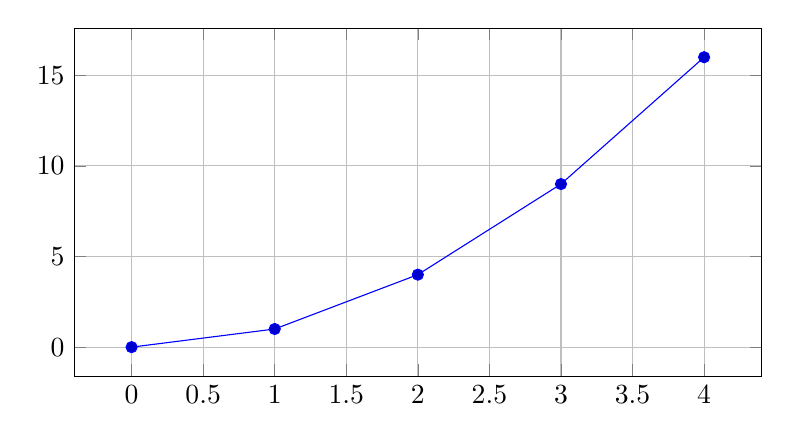
\begin{tikzpicture}
\begin{axis}[
    width=0.85\linewidth,
    height=6cm,
    grid=major
]
\addplot coordinates {(0,0) (1,1) (2,4) (3,9) (4,16)};
\end{axis}
\end{tikzpicture}
\caption{Crecimiento cuadrático}
\end{figure}

%
\section{Gráficos múltiples}%
\label{sec:Grficosmltiples}%

\begin{figure}[H]
\centering
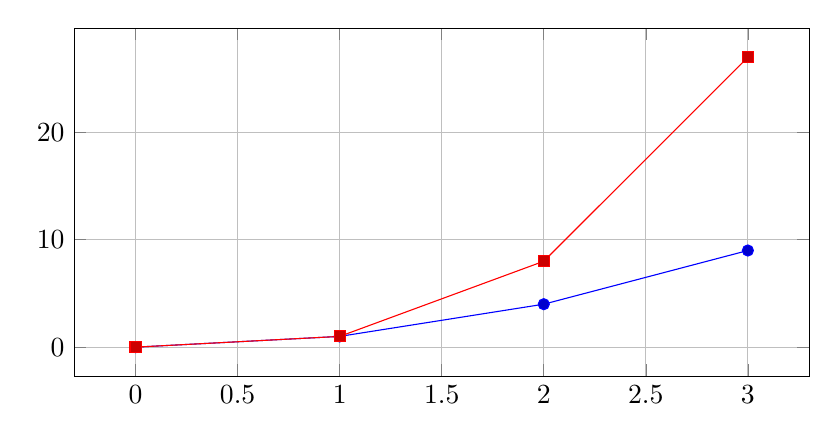
\begin{tikzpicture}
\begin{axis}[
    width=0.9\linewidth,
    height=6cm,
    grid=both
]
\addplot coordinates {(0,0) (1,1) (2,4) (3,9)};\addplot coordinates {(0,0) (1,1) (2,8) (3,27)};
\end{axis}
\end{tikzpicture}
\caption{Comparación de funciones}
\end{figure}

%
\newpage%
Contenido en una nueva página.%
\end{document}